\documentclass[12pt]{article}
\usepackage{amssymb, amsmath}
\usepackage{fancyhdr,lastpage}
\usepackage{amsmath,amsfonts,amssymb}
\usepackage{graphicx}
\usepackage{stix}
\usepackage{enumitem}
\usepackage{listings}
\tolerance 10000
\headheight 0in
\headsep 0in
\evensidemargin 0in
\oddsidemargin \evensidemargin
\textwidth 6.5in
\topmargin .25in
\textheight 8.7in

\usepackage{listings}
\usepackage{color}
 
\definecolor{codegreen}{rgb}{0,0.6,0}
\definecolor{codegray}{rgb}{0.5,0.5,0.5}
\definecolor{codepurple}{rgb}{0.58,0,0.82}
\definecolor{backcolour}{rgb}{0.95,0.95,0.92}
 

\lstdefinestyle{mystyle}{
    backgroundcolor=\color{backcolour},   
    commentstyle=\color{codegreen},
    keywordstyle=\color{magenta},
    numberstyle=\tiny\color{codegray},
    stringstyle=\color{codepurple},
    basicstyle=\footnotesize,
    breakatwhitespace=false,         
    breaklines=true,                 
    captionpos=b,                    
    keepspaces=true,                 
    numbers=left,                    
    numbersep=5pt,                  
    showspaces=false,                
    showstringspaces=false,
    showtabs=false,                  
    tabsize=2
}

\lstset{style=mystyle}


\newcommand{\CC}{{\mathbb C}}
\newcommand{\QQ}{{\mathbb Q}}
\newcommand{\RR}{{\mathbb R}}
\newcommand{\ZZ}{{\mathbb Z}}
\newcommand{\NN}{{\mathbb N}}
\newcommand{\FF}{{\mathbb F}}


\newcommand{\Zerobold}{{\boldsymbol 0}}
\newcommand{\Onebold}{{\boldsymbol 1}}
\newcommand{\xbold}{{\boldsymbol x}}

\newcommand{\mfrak}{{\mathfrak m}}

\newcommand{\Acal}{{\mathcal A}}
\newcommand{\Ncal}{{\mathcal N}}
\newcommand{\Pcal}{{\mathcal P}}
\newcommand{\Qcal}{{\mathcal Q}}

\newcommand{\sqbinom}[2]{\genfrac{[}{]}{0pt}{}{#1}{#2}}
\newcommand{\angbinom}[2]{\genfrac{\langle}{\rangle}{0pt}{}{#1}{#2}}

\newcommand{\qddx}{(d/dx)_{q}}

%\newcommand{\pfcl}{\emph{Proof of claim}}
\newenvironment{proof}{\paragraph{Proof: }}{\hfill$\blacksquare$}



\def\multiset#1#2{\ensuremath{\left(\kern-.3em\left(\genfrac{}{}{0pt}{}{#1}{#2}\right)\kern-.3em\right)}}


\DeclareMathOperator{\des}{des}
\DeclareMathOperator{\maj}{maj}
\DeclareMathOperator{\ev}{ev}
\DeclareMathOperator{\Hom}{Hom}
\DeclareMathOperator{\trace}{tr}
\DeclareMathOperator{\inv}{inv}

\newtheorem{problem}{Problem}%[section]

\begin{document}

\begin{center}
{\bf Julio Soldevilla}
\\
{\bf EECS 545 Winter 2018 --- Problem Set 4 }
\end{center}

\begin{problem}
\normalfont
Problem 1
\end{problem}

\begin{proof}

\begin{enumerate}
\item After running the code for problem 1.a, we get that the energy for image 1 is $36$ and the energy for image 2 is $42$, according to the Potts Model and we get the following images:

\begin{figure}[!htbp]
\centering
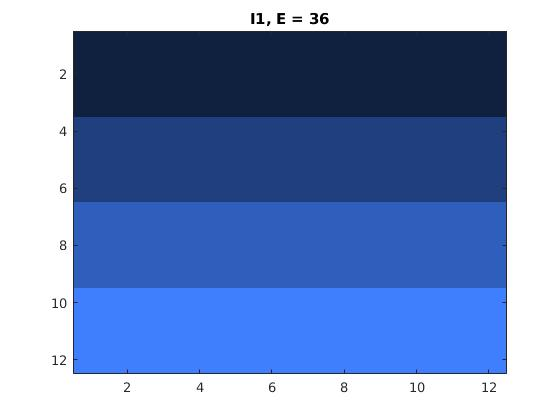
\includegraphics[width=8cm]{prob1_a_im1.jpg}
\caption{}
\end{figure}

\begin{figure}[!htbp]
\centering
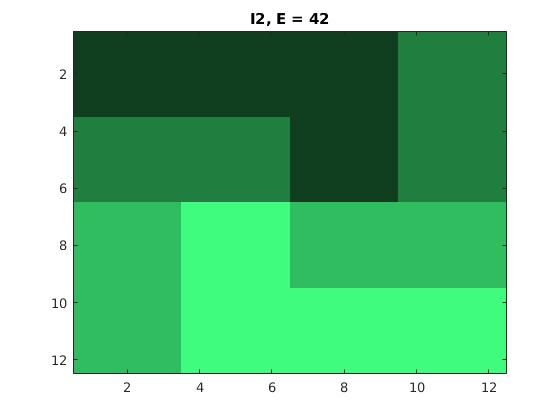
\includegraphics[width=8cm]{prob1_a_im2.jpg}
\caption{}
\end{figure}

The code of problem 1.a is: 

\lstinputlisting[language=Matlab]{potts.m}

\item After running the code for problem 1.b, we get that the energy of the image following the Mumford Shah model is $67.6103$. The code for this problem is:

\lstinputlisting[language=Matlab]{mumford_shah.m}

\item In the equation above, we can see that the boundary terms comes from the pott's model. Also, we can split the image (the squared difference of images) in the problem into regions based on the pixel values on each of the regions. However, given the images we have, each region would have its own unique minimum. Thus, since each region has its own minimum, we cannot say that the f-hat given is the minimizer of the whole image. All we can do to in a sense minimize the energy in the image is to minimize the sum of the energies in each part of the regions. Thus minimize the double integral and the boundary term.

\end{enumerate}

\end{proof}


\begin{problem}
\normalfont
Problem 2
\end{problem}


\begin{proof}
\begin{enumerate}
\item For part a of problem 2.1, after running the q1.m file we get the following output

\begin{figure}[!htbp]
\centering
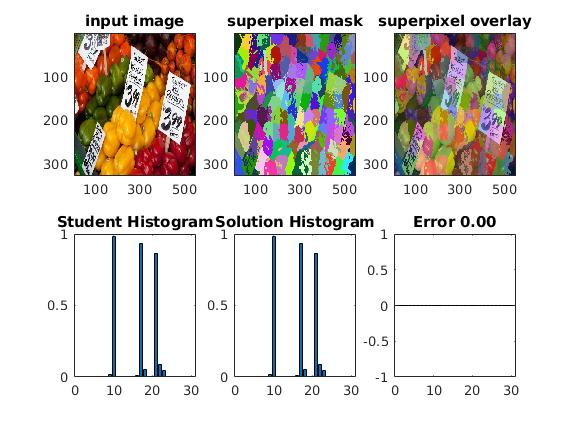
\includegraphics[width=18cm]{problem2_1.jpg}
\caption{Problem 2.1}
\end{figure}

If we just show the 88 superpixel from the figure (the superpixel used to compute the histograms), we can see that it corresponds to one of the yellow peppers that is right below the $3.99$ dollar sign.

\item  This is problem 2 part 2

\begin{enumerate}
\item For part a of problem 2.2, after running the q2.m file we get the following output:

\begin{figure}[!htbp]
\centering
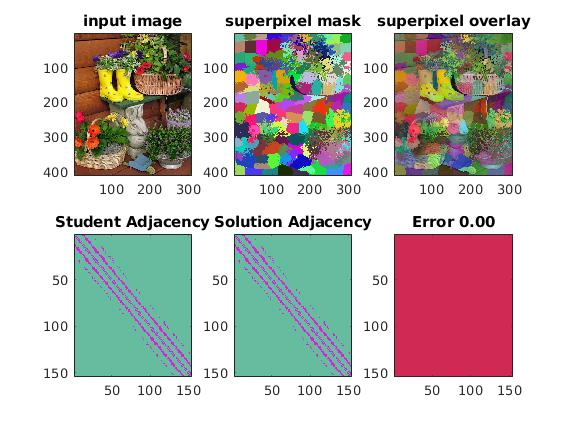
\includegraphics[width=18cm]{problem2_2.jpg}
\caption{Problem 2.2 part a}
\end{figure}

\item This is part b of problem 2.2. The average node degree is $8.8571$. The code for computing this is:

\lstinputlisting[language=Matlab]{node_degree.m}

\item This is part c of problem 2.2. The adjacency graph is not a perfect banded diagonal matrix because of two reasons: first of all, if the adjacency graph was a perfect banded diagonal matrix, then that would imply that every superpixel would have the same number of adjacent edges and second of all, it would imply that if superpixel i was neighbor with superpixels $(i + 1, ..., i+j)$ for some real number $j$, then super pixel $i + 1$ would be neighbor with superpixels $(i+2,..., i+(j+1))$, so basically the indices of the superpixels and their neighbors would increase linearly for all the superpixels. In this case, we can see from the picture of superpixels, that the superpixels obtained clearly don't satisfy these conditions, not every superpixel has the same number of neighbors and we can probably inspect the code to see that the indices of the superpixel and their neighbors don't increase as was described above. Because of these reasons, we see that why we don't obtain a perfect banded diagonal matrix.

\end{enumerate}

\item This is problem 2 part 3

\begin{enumerate}

\item For part a of problem 2.3 after running the q3.m file we get the following output in figure 5:

\begin{figure}[!htbp]
\centering
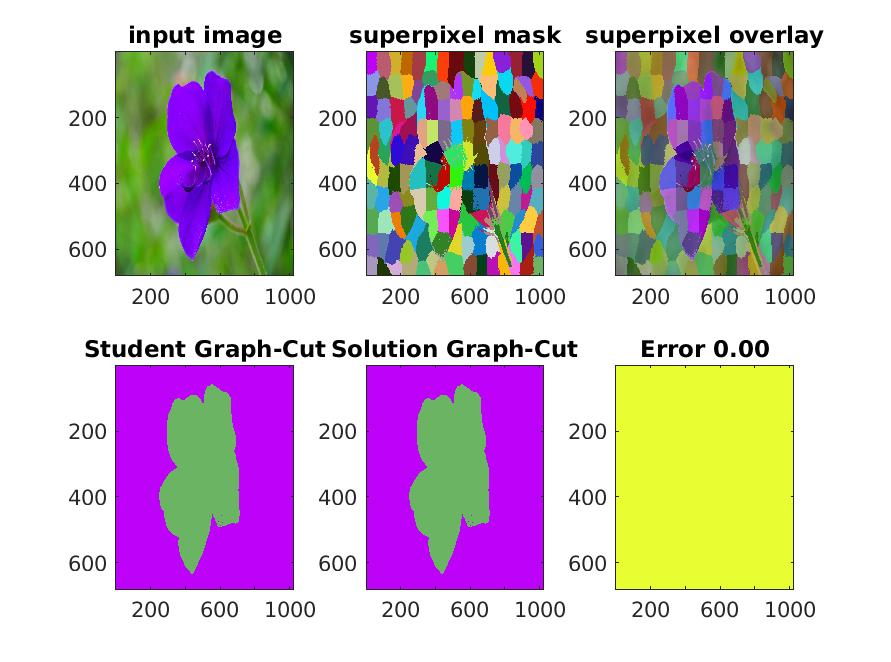
\includegraphics[width=18cm]{problem_2_3b.jpg}
\caption{Problem 2.3 part a}
\end{figure}

\item This is part b of problem 2.3. This is an image of the capacity matrix before running graph cuts, shown in figure 6:

\begin{figure}[!htbp]
\centering
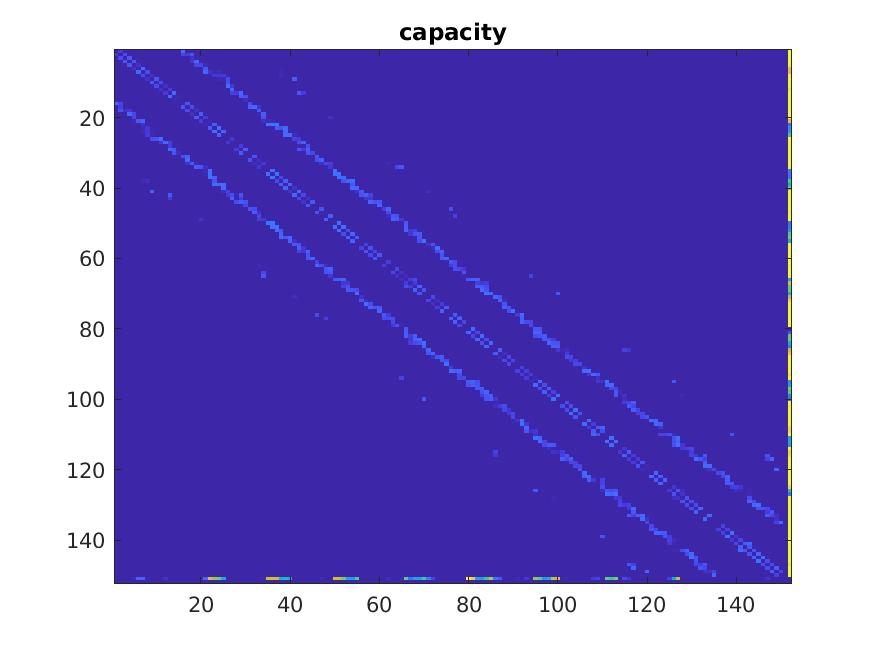
\includegraphics[width=18cm]{capacity_2_3b.jpg}
\caption{Problem 2.3 part b}
\end{figure}

We can clearly see that the capacity image is related to the adjacency in the sense that the capacity has a very big $105 \times 150$ window that is also an (almost perfect) banded diagonal matrix. Also, we can see that whereas in the adjacency matrix the entries of the matrix are either 0 or 1, in the capacity matrix we have entries that can bee between 0 and 1 and so we can see some of the possible weights that the edges between the superpixels can have. Finally, we can see that the capacity matrix is of size bigger than $150 \times 150 $ and from the formulation of this matrix and looking at the left and down edges of the image, we can see that these capacities correspond to the capacity of the edges connecting the source (on the right part of the matrix) and the capacity of the edges on the edges connectin with the sink (on the bottom part of the matrix). These rows and columns related to the source and sink of the graph are clearly recognizable from the capacity image.  

 \item This is problem 2.3 part c. In this problem, we are downeighting the capacity between vertices (not considering the source and the sink) or in a sense having higher capacity between any edge and the source or sink compared connection between edges because in this way we are reducing the probability that when we compute the residual graph, we run out of edges (basically having edges of capacity 0) from the source (or sink) to any other edge in the graph. Also, by downweighting the capacity in edges between non sink and non source vertices, then we are reducing the probability that the cut in our graph goes through edges connecting the source or the sinnk to any other edge, since these edges will in general have higher capacity and so a higher chance of a higher flow than the edges between non source vertices. Thus, this reduces the probability that we lose connections from the source or sink to the rest of the graph.

\end{enumerate}

\item For problem 2 part 4 we have the following results: 

\begin{enumerate}

\item This is the output we get from running the example.m file once:

\begin{figure}[!htbp]
\centering
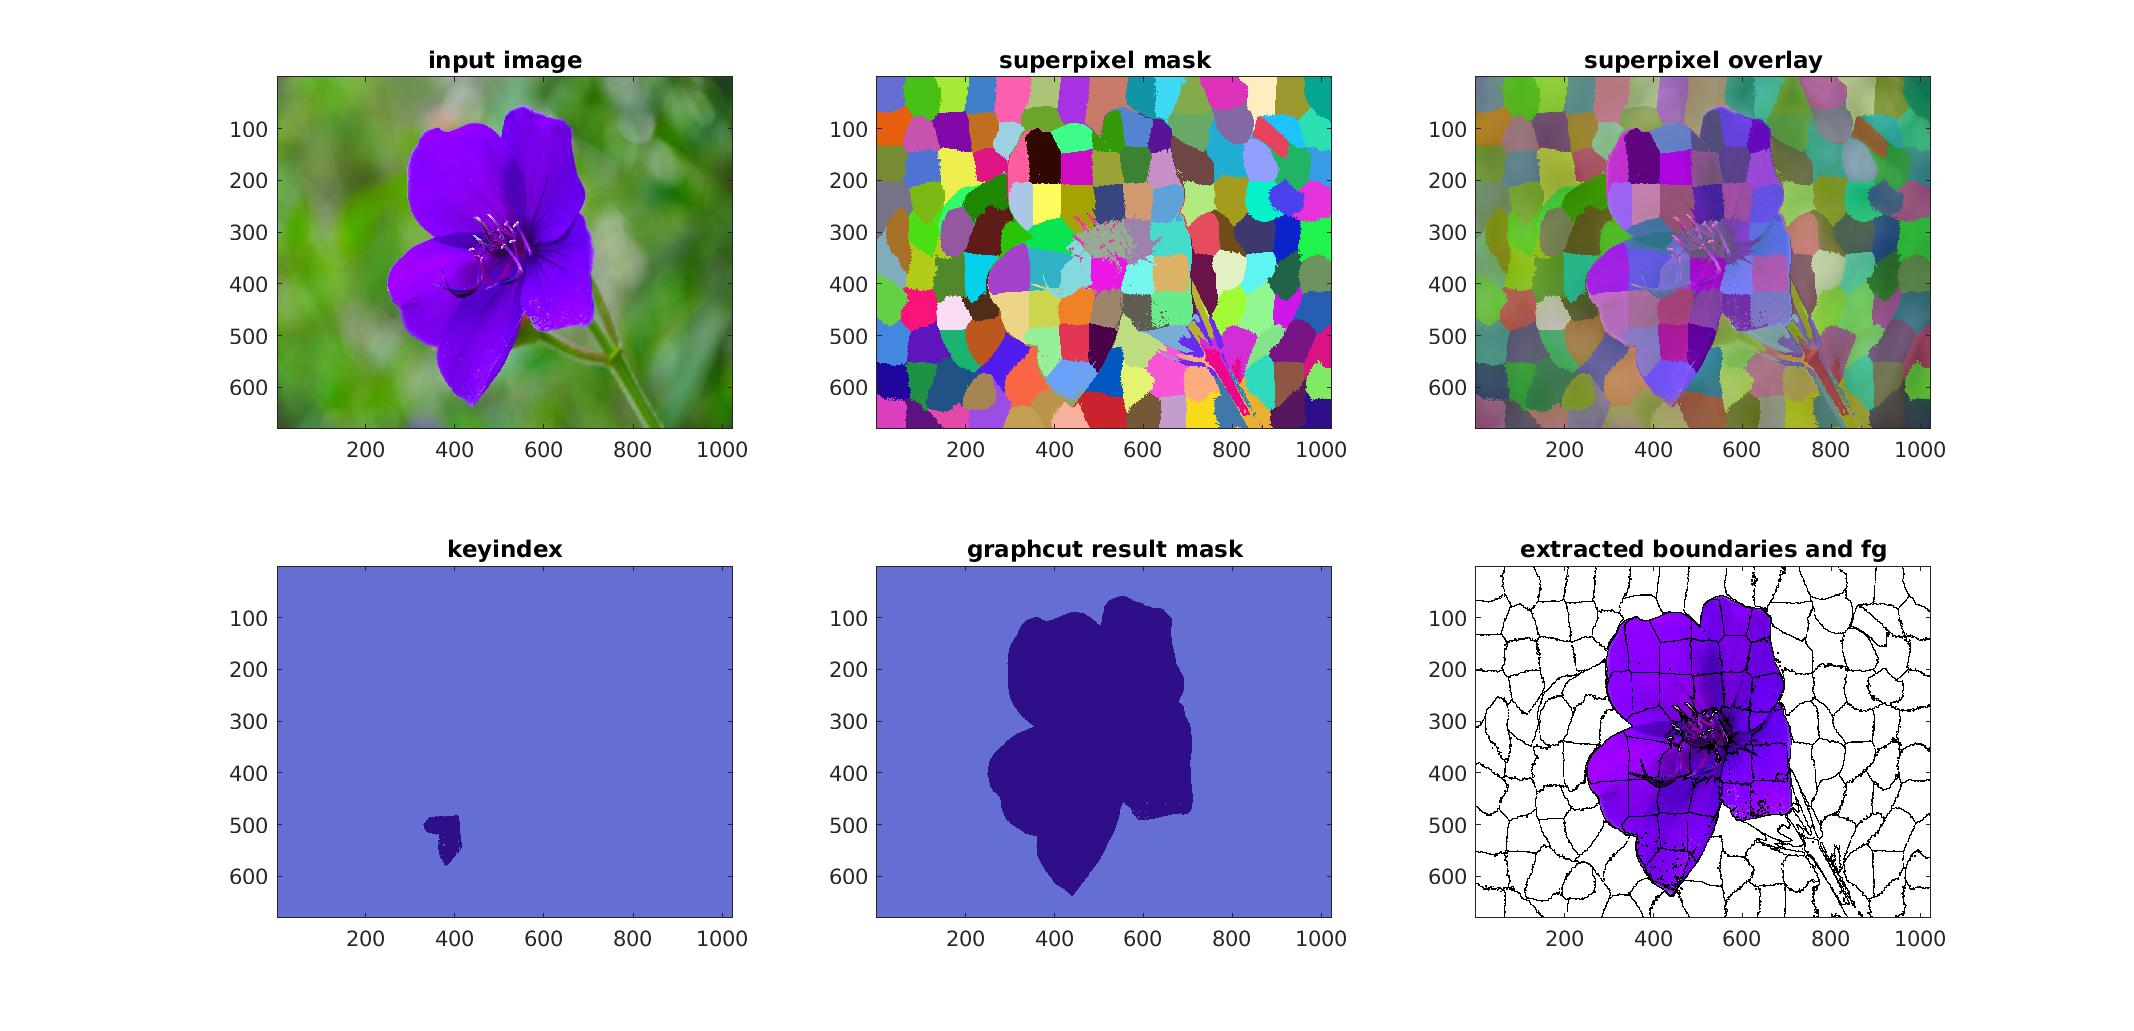
\includegraphics[width=18cm]{problem2_4a.jpg}
\caption{Problem 2.4 a}
\end{figure}

\item This is the output for running the example.m file with the flag image:

\begin{figure}[!htbp]
\centering
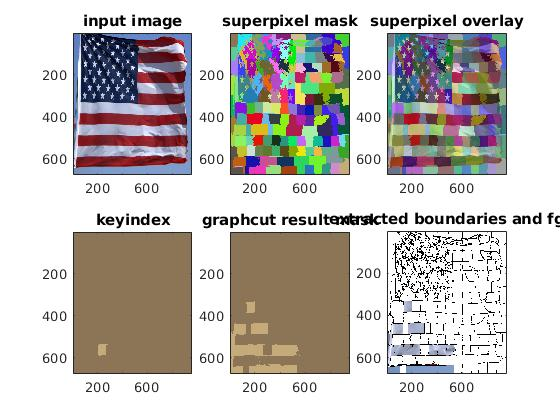
\includegraphics[width=18cm]{problem2_4b.jpg}
\caption{Problem 2.4 b}
\end{figure}

In this figure, I didn't get the whole stripe. I think to getting just one stripe (either white or red) is hard because of two reasons: First, getting just one stripe of the flag is hard because (even though there are some shadows in the picture), the white stripes or red stripes in the flag have a very similar color histogram on average (either with variations of white or variations of red) and so this will make it difficult to get just one stripe. Now, it is also hard to get a whole stripe (either white or red), because along one stripe there is also a good amount of variation in the color of the stripe because of the shadows of the flag. Thus, this would mean there are also different color histograms along one stripe of the flag which would make it difficult to get just one stripe of the flag. 

\item This is the output for running the example.m file with the basket image and trying to get the boots in the foreground:

\begin{figure}[!htbp]
\centering
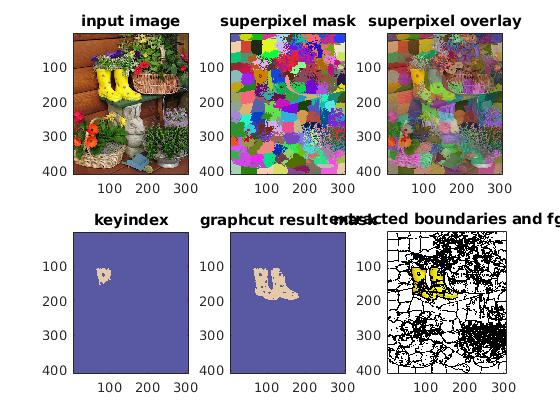
\includegraphics[width=18cm]{problem2_4c.jpg}
\caption{Problem 2.4 c}
\end{figure}

In this part of the problem, I didn't get the whole boots, I missed the pattern on the boots. In this case, I think I didn't get the whole boots image because the pattern on the boots has very different color and so it will have a very different color histogram. Thus, when doing the graph cut, these regions of the pattern will be on the other end of the cut, not where the boots are. Also, maybe the pattern of the flowers (not smooth regions) makes it more difficult to recognize them as part of the boots. 

\item This is the output for running the example.m file with the basket image and trying to get the basket in the foreground:

\begin{figure}[!htbp]
\centering
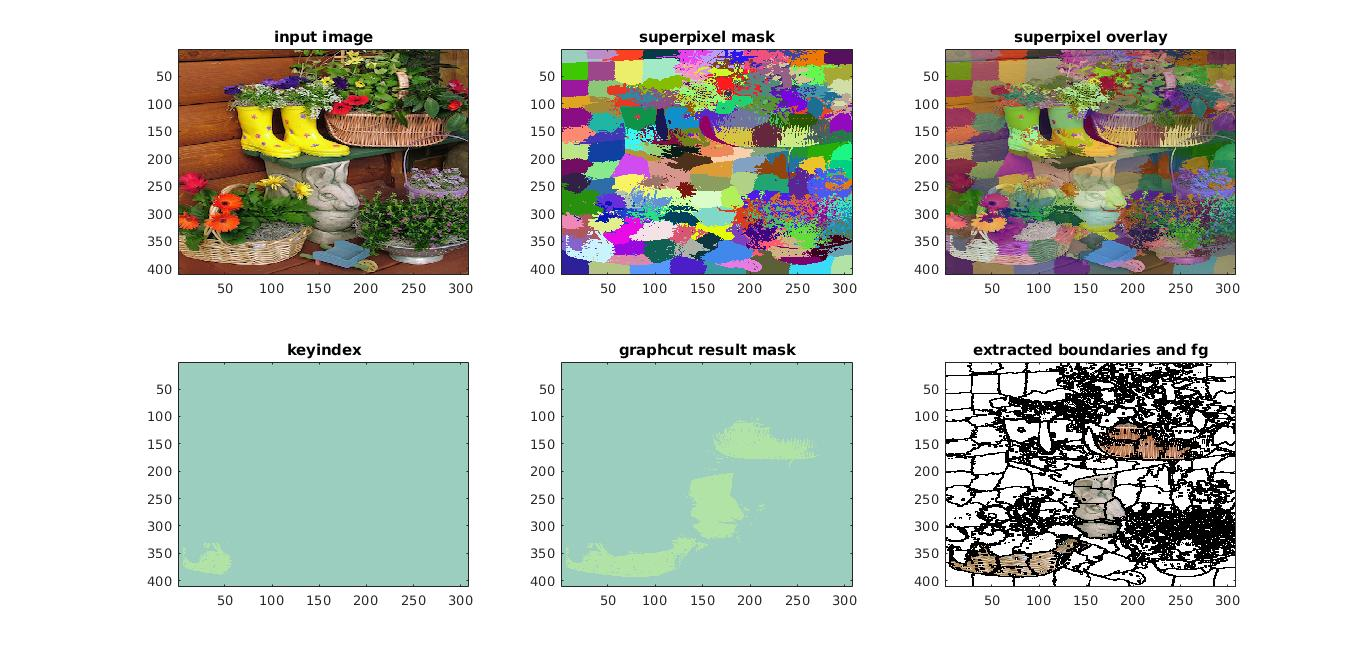
\includegraphics[width=18cm]{problem2_4d_both_baskets.jpg}
\caption{Problem 2.4 d}
\end{figure}

In this region I didn't get thw whole basket. In the system we have, I would change the bin size in the histogram to be more sensitive to variations in color. In my images, I distinguished parts of the basket but also parts of the rabbit and parts of the other basket. In this case, I think what is happening is that because of the width of the bins in the histograms, we are probably putting together the color of the rabbit and the baskets and so that's why we are getting all these regions. To get more of the basket and less of the rabbit or the other basket, increasing the bin of the histogram would help us detect better the color on the basket. 

\end{enumerate}

\end{enumerate}
\end{proof}


\begin{problem}
\normalfont
Problem 3
\end{problem}

\begin{proof}

\begin{enumerate}
\item For this image, we see the default result, with hyperparameter $k = 4$ is:

\begin{figure}[!htbp]
\centering
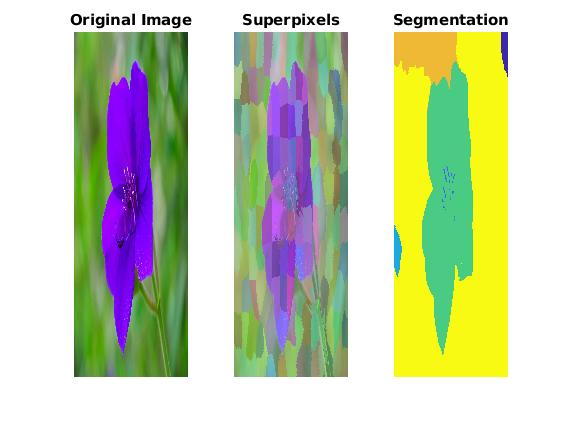
\includegraphics[width=14cm,height = 10cm]{max_flower_4.jpg}
\caption{Problem 3.1 a, k =4}
\end{figure}


\item In this problem, we computed the weights differently because first of all, in problem 3.1, we are not working with a graph cut and so we don't have a source or sink edge. Thus, we don't have the need to increase the probability of not losing some edges (in problem 2 we wante to save many edges conected to source or sink). Thus, we don't need to downweight any edge capacity. 

\item For this problem, after implementing the post - processing we get:

\begin{figure}[!htbp]
\centering
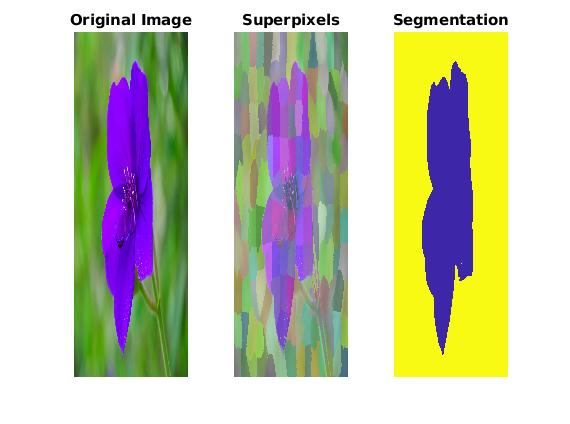
\includegraphics[width=14cm,height = 10cm]{max_flower_4_post_pro.jpg}
\caption{Problem 3.1 c, k =4}
\end{figure}

The implementation of the function is the following, it is the whole code for fh.m, but the important part implementing this function is in the final lines of code.

\lstinputlisting[language=Matlab]{fh.m}

\item Finally, after commenting out the post - processing function, we can play around with the parameter $k$ and we get the following results:

\begin{figure}[!htbp]
\centering
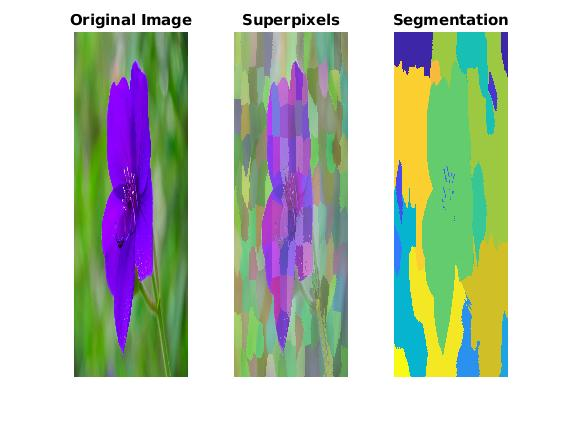
\includegraphics[width=14cm,height = 10cm]{max_flower_1.jpg}
\caption{Problem 3.1 a, k = 1}
\end{figure}


\begin{figure}[!htbp]
\centering
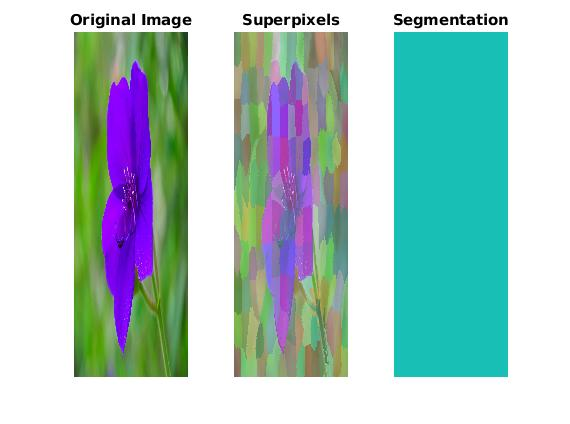
\includegraphics[width=14cm,height = 10cm]{max_flower_20.jpg}
\caption{Problem 3.1 a, k = 20}
\end{figure}


We can see that as we change the value of $k$, then the higher the value of $k$ we don't get as many components but we get a primitive shadow of the main things of the picture, in this case the petals of the flower. As $k$ decreases, we get many more components and some more details of the picture, in this case the pistils (the thingies in the center of the flower). So $k$ is playing a role of quantity of components in the algorithm (and in a sense the level of detail we can see). The lower the $k$ the more components. This makes sense sinse $k$ is some element in the condition for combining components or not.

\end{enumerate}
\end{proof}

\end{document}